\documentclass[conference]{IEEEtran}
\IEEEoverridecommandlockouts

\usepackage{cite}
\usepackage{amsmath,amssymb,amsfonts}
\usepackage{graphicx}
\usepackage{textcomp}
\usepackage{xcolor}
\usepackage{booktabs}
\usepackage{array}
\usepackage{hyperref}
\usepackage{balance}

\hypersetup{
    colorlinks=true,
    linkcolor=blue,
    citecolor=blue,
    urlcolor=blue
}

\begin{document}

\title{Sample-Efficient Meta-Learning for Recommender System Algorithm Selection: A Ranking-Centric Analysis}

\author{
    \IEEEauthorblockN{Hirok Jyoti Dewri}
    \IEEEauthorblockA{
        \textit{Department of Computer Science and Engineering}\\
        \textit{Tezpur University}\\
        Tezpur, Assam, India\\
        csp26001@tezu.ernet.in
    }
    \and
    \IEEEauthorblockN{Dr. Tribikram Pradhan}
    \IEEEauthorblockA{
        \textit{Department of Computer Science and Engineering}\\
        \textit{Tezpur University}\\
        Tezpur, Assam, India\\
        tribikram@tezu.ernet.in
    }
}

\maketitle

\begin{abstract}
In recommender systems, algorithm selection is important but computationally expensive. It is difficult for users and developers to select appropriate algorithms for specific datasets while dealing with millions of user interactions and testing multiple algorithms. Therefore, we present AutoRecSys, a sample-efficient meta-learning framework for algorithm selection that operates on small subsamples of data. Using a Random Forest meta-model, AutoRecSys predicts which algorithm would yield the best Top-K ranking performance (NDCG@10) based on 29 lightweight statistical meta-features derived from a subsample of $N$ ratings. Thirteen real-world datasets covering sparse retail, cold-start, and dense interaction scenarios are used to evaluate AutoRecSys under strict data leakage protection. Our experiments show that early selection using only 250 ratings achieves equivalent end-to-end recommendation quality to full-data selection---formally confirmed through Two One-Sided Tests (TOST) equivalence testing ($p < 0.0001$)---while providing a median speedup of $941\times$ over the traditional approach of training all candidate algorithms. Additionally, we integrate Parameter-Efficient Fine-Tuning (PEFT) via LoRA \cite{hu2022lora} into both the neural collaborative filtering component and the meta-learner, demonstrating that transfer learning with low-rank adapters can improve neural recommender sample efficiency while training only a fraction of the model parameters. Overall, our results demonstrate that effective algorithm selection does not require the full dataset: a small subsample and a pre-trained meta-model are sufficient, reducing selection time from minutes to under one second.
\end{abstract}

\begin{IEEEkeywords}
algorithm selection, meta-learning, recommender systems, AutoML, NDCG@10, sample efficiency, collaborative filtering, parameter-efficient fine-tuning, LoRA
\end{IEEEkeywords}

%------------------------------------------------------------
\section{Introduction}
%------------------------------------------------------------

Recommender systems are an integral part of the modern internet. They shape how users discover products, explore content, and engage on social platforms. These systems can be constructed using a variety of techniques, including deep learning methods such as NCF \cite{he2017ncf}, matrix factorization methods such as SVD and NMF \cite{koren2009matrix}, and neighbourhood-based methods such as KNN \cite{sarwar2001item}. Some methods focus on finding similarities between users or items, while others learn patterns from the entire dataset.

However, a key challenge is deciding which algorithm is most suitable for a new dataset. The traditional approach is to train and test multiple candidate algorithms, which is time-consuming. Moreover, real-world datasets often contain millions of interactions, so training complex models such as SVD++ \cite{koren2008factorization} can take considerable time. Because of this, developers and researchers often rely on guesswork, default choices, or evaluation metrics that may not fully reflect recommendation quality, resulting in suboptimal decisions.

To address this, we introduce AutoRecSys, a sample-efficient meta-learning framework for algorithm selection. Instead of using the full dataset, this framework works with a subsample, typically ranging from 250 to 10,000 ratings, and extracts simple features from it. These features are then used in a Random Forest model to predict which algorithm will perform better in terms of ranking quality (NDCG@10) \cite{jarvelin2002ndcg}. The core hypothesis is that basic structural properties of a dataset, such as sparsity and interaction density, stabilize quickly and are sufficient to distinguish between scenarios where different algorithm families are most effective.

Importantly, we evaluate performance using NDCG@10 \cite{jarvelin2002ndcg} rather than traditional metrics such as RMSE \cite{koren2009matrix}. This shift shows that simpler methods, such as KNN \cite{sarwar2001item}, can outperform more complex models in certain scenarios \cite{cremonesi2010performance}, which challenges some common assumptions in the literature.

Our main contributions are:
\begin{itemize}
    \item A meta-learning framework for selecting recommendation algorithms based on ranking performance rather than prediction error.
    \item Evidence that a small data sample (as low as 250 ratings) can support effective algorithm selection, with formal equivalence to full-data selection established through TOST testing \cite{schuirmann1987tost}.
    \item A computational cost analysis showing a median $941\times$ speedup over exhaustive algorithm evaluation.
    \item An interpretability analysis showing that simple features, such as user rating behaviour, play an important role in algorithm selection.
    \item Integration of Parameter-Efficient Fine-Tuning (PEFT) via LoRA \cite{hu2022lora} into both the neural recommender and meta-learner components, demonstrating that transfer learning with low-rank adapters improves sample efficiency for neural collaborative filtering.
\end{itemize}

%------------------------------------------------------------
\section{Related Work}
%------------------------------------------------------------

\subsection{Algorithm Selection and AutoML}

The problem of algorithm selection was first introduced by Rice \cite{rice1976algorithm}, where the goal is to map dataset characteristics to the performance of different algorithms. This idea directly forms the basis of our work.

In recent years, AutoML systems such as Auto-Sklearn \cite{feurer2015autosklearn} and studies like Hutter et al. \cite{hutter2019automl} have applied this concept using meta-learning, where past performance and dataset features are used to guide selection. However, these approaches are designed for general machine learning problems and do not specifically consider recommender systems.

In collaborative filtering, factors such as sparsity and user-item interaction patterns play a major role in determining algorithm performance. These aspects are not explicitly handled in general AutoML systems, which motivates the need for a more focused approach like AutoRecSys.

\subsection{Meta-Learning in Recommender Systems}

Among existing works, Cunha et al. \cite{cunha2018metalearning} is the closest to our approach. They use meta-learning to select collaborative filtering algorithms based on dataset features. However, their work focuses on prediction accuracy using RMSE and assumes access to the full dataset for feature extraction.

In contrast, our approach differs in two key ways. First, we use a ranking-based metric (NDCG@10), which better reflects recommendation quality. Second, we extract meta-features from small subsamples ($N = 250$ to $10,000$), making the approach more efficient.

Other works such as Lemke et al. \cite{lemke2015metalearning} and Vanschoren \cite{vanschoren2018meta} provide a general overview of meta-learning, but they do not focus on sample efficiency in recommender systems. Finn et al. \cite{finn2017maml} propose MAML, which enables fast adaptation of model parameters. However, our approach is different, as we do not adapt a single model but instead select the best algorithm from a fixed set of candidates.

\subsection{Collaborative Filtering Methods}

In this work, we consider a set of commonly used collaborative filtering algorithms covering different approaches. Content-based approaches, which rely on item attributes rather than user interactions, are not considered here as AutoRecSys targets collaborative filtering settings exclusively \cite{pazzani2007content}. Neighbourhood-based methods \cite{ekstrand2011cf, linden2003amazon, sarwar2001item}, such as KNN, rely on similarity between users or items and are known to perform well in sparse datasets. Matrix factorization methods \cite{koren2008factorization, koren2009matrix}, such as SVD and NMF, learn latent representations from the rating matrix and generally require more data to perform well. SVD++ \cite{koren2008factorization} extends this by incorporating implicit feedback, but it also increases computational complexity.

Neural approaches like NCF \cite{he2017ncf} can model complex and nonlinear interactions, but they typically require large amounts of data. Session-based methods \cite{hidasi2016session} are not considered in this work because they depend on sequential interaction data, which is not available in our datasets.

Previous studies such as Tikk et al. \cite{tikk2009study} and Cremonesi et al. \cite{cremonesi2010performance} have shown that simpler methods can sometimes outperform more complex models in top-N recommendation tasks. This observation supports our focus on ranking performance using NDCG@10.

\subsection{Ranking-Based Evaluation}

Traditionally, RMSE has been widely used for evaluating recommender systems \cite{koren2009matrix}. However, it mainly measures prediction error and does not reflect the quality of top-N recommendations.

Cremonesi et al. \cite{cremonesi2010performance} showed that a lower RMSE does not always lead to better ranking performance. J\"{a}rvelin and Kek\"{a}l\"{a}inen \cite{jarvelin2002ndcg} introduced NDCG as a ranking metric that considers both relevance and position of items.

Further, Krichene and Rendle \cite{krichene2020sampled} highlighted that certain evaluation methods can introduce bias if not properly designed.

Based on these observations, we use NDCG@10 as our main evaluation metric. This choice aligns better with real-world recommendation scenarios and differentiates our work from previous algorithm selection approaches that rely on RMSE \cite{cunha2018metalearning}.

\subsection{Parameter-Efficient Fine-Tuning}

Recent advances in parameter-efficient fine-tuning (PEFT) have demonstrated that large pre-trained models can be effectively adapted to new tasks by training only a small number of additional parameters \cite{hu2022lora, houlsby2019adapters, li2021prefix}. LoRA (Low-Rank Adaptation) \cite{hu2022lora} is a particularly effective approach that injects trainable low-rank decomposition matrices into existing model layers while keeping the original weights frozen. This reduces the number of trainable parameters significantly while preserving the knowledge from pre-training.

While PEFT methods have primarily been applied to natural language processing and computer vision, their application to recommender systems remains largely unexplored. In this work, we integrate LoRA into both the neural collaborative filtering component (NCF) and the meta-learner, investigating whether transfer learning via PEFT can improve sample efficiency in the recommendation setting.

\subsection{Model Interpretability}

Understanding why a model makes a particular decision is important, especially in algorithm selection. In this work, we use SHAP \cite{lundberg2017shap}, which is based on Shapley values, to measure the contribution of each feature.

By applying SHAP to our Random Forest meta-model, we identify which dataset characteristics influence the selection of algorithms. This helps us not only achieve good performance but also provide insight into how and why certain algorithms are preferred under different conditions.

%------------------------------------------------------------
\section{Methodology}
%------------------------------------------------------------

\subsection{Framework Overview}

AutoRecSys consists of three major steps: (1) Subsampling, (2) Feature Extraction, and (3) Algorithm Selection. The features are first extracted from only a small portion of the data. A trained meta-learning model then uses these features to predict the best algorithm.

To prevent data leakage during meta-dataset construction and evaluation, we implement a strict partitioning protocol. For each dataset, a train/test split is applied first. Meta-features are extracted exclusively from the training split, and candidate algorithms are evaluated on the test split. Thus, the test split is completely unseen during feature extraction and selection.

The overall pipeline is shown in Fig.~\ref{fig:framework}. The offline meta-learning phase trains the Random Forest on historical datasets using NDCG@10 per dataset per algorithm as oracle labels. The online inference phase takes a new dataset, subsamples $N$ ratings from the training split, extracts 29 meta-features, and predicts the best algorithm.

\begin{figure}[htbp]
    \centering
    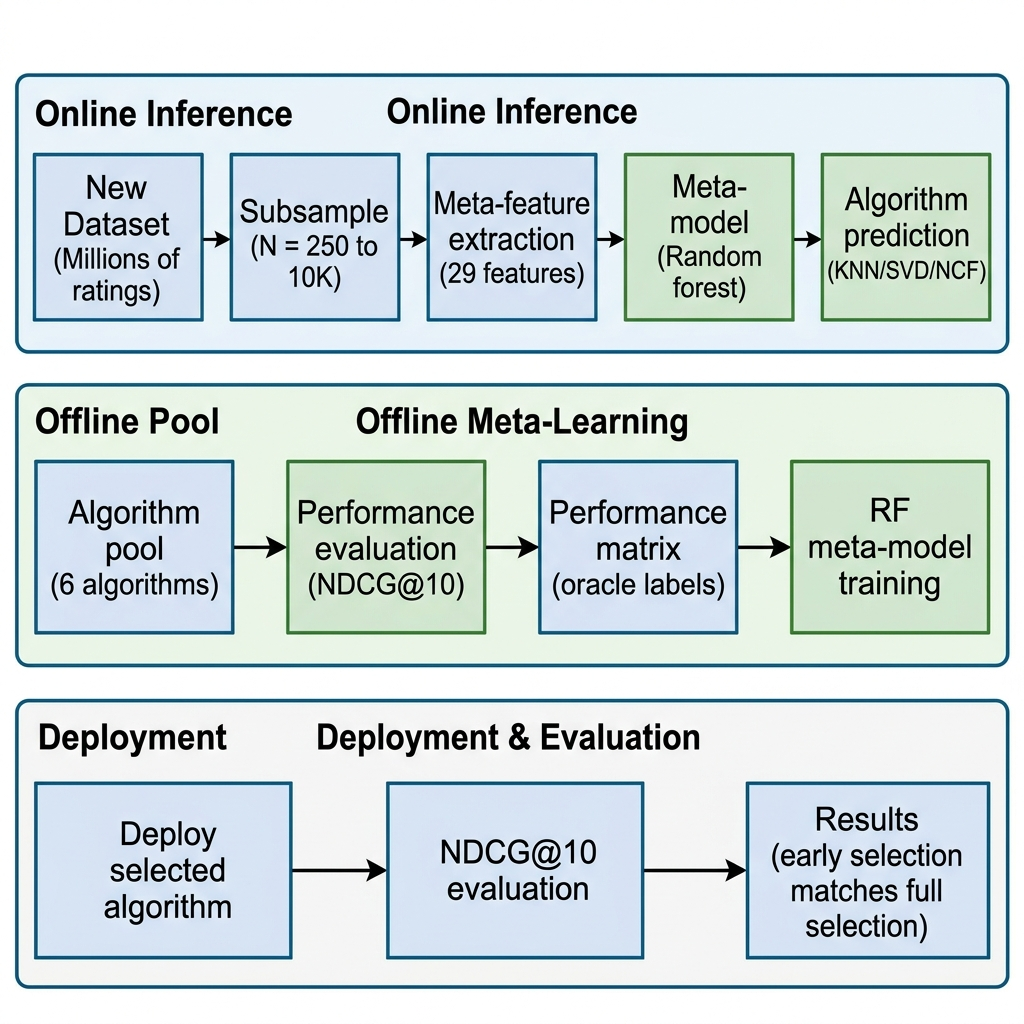
\includegraphics[width=\columnwidth]{fig1_framework.png}
    \caption{AutoRecSys pipeline. Top: online inference using a subsample of $N = 250$ to $10$K ratings. Middle: offline meta-learning on historical datasets. Bottom: deployment and NDCG@10 evaluation showing early selection matches full-data selection at 60\% accuracy.}
    \label{fig:framework}
\end{figure}

\subsection{Algorithm Selection Strategy}

The algorithm selection process in AutoRecSys is guided by dataset characteristics extracted from a small subsample. The meta-model (Random Forest) learns to map these characteristics to the most suitable recommendation algorithm.

In addition to the learned model, we can interpret the selection behaviour under different dataset scenarios as follows. For sparse datasets (high sparsity, low ratings per user), neighbourhood-based methods such as KNN are preferred, as they rely on local similarity and perform well with limited interactions. For dense datasets (low sparsity, high interaction volume), matrix factorization methods such as SVD and SVD++ are more effective, as they can learn meaningful latent representations from sufficient data. For cold-start scenarios, KNN-based approaches are more suitable since they do not require extensive historical data. For datasets with high rating variability, factorization-based methods such as NMF and SVD are preferred due to their ability to capture complex rating patterns.

These scenario-based interpretations align with the feature importance analysis, where sparsity, average ratings per user, and rating variance play a key role in determining algorithm performance. Thus, the meta-learning model implicitly captures these relationships and enables efficient algorithm selection without exhaustive training of all candidate models.

\subsection{PEFT-Enhanced Neural Collaborative Filtering}

We extend the NCF algorithm \cite{he2017ncf} with LoRA-based parameter-efficient fine-tuning \cite{hu2022lora} to investigate whether transfer learning can improve sample efficiency for neural recommenders. The approach follows a two-phase strategy:

\textbf{Phase 1 --- Pre-training.} A base NCF model is trained on a large source dataset (MovieLens-1M, $\sim$1 million ratings) using the standard MLP architecture with embedding dimension 32 and hidden layers $[64, 32, 16]$. This phase captures general user--item interaction patterns that transfer across domains.

\textbf{Phase 2 --- LoRA Adaptation.} For each target dataset, the pre-trained MLP weights are frozen, and low-rank adapter matrices ($r = 8$, $\alpha = 16$) are injected into each linear layer. New user and item embeddings are initialized for the target vocabulary. Only the LoRA parameters and the new embeddings are trained, reducing the number of trainable parameters to a fraction of the full model.

This design is motivated by the observation that MLP layers in NCF learn general nonlinear interaction patterns that are largely domain-agnostic, while embeddings encode dataset-specific user and item identities. By transferring the MLP and adapting via LoRA, we hypothesize that PEFT-NCF can achieve competitive performance with fewer training samples and epochs compared to training NCF from scratch.

%------------------------------------------------------------
\section{Experimental Results}
%------------------------------------------------------------

\subsection{RQ1: Algorithm Diversity under NDCG@10}

The performance of all algorithms is compared across datasets using NDCG@10, as shown in Table~\ref{tab:rq1}.

\begin{table}[t]
\centering
\caption{NDCG@10 of each algorithm on each dataset. Best results per dataset in \textbf{bold}.}
\label{tab:rq1}
\small
\begin{tabular}{lcccccc}
\toprule
Dataset & KNN & NCF & NMF & SVD & SVDpp & SlopeOne \\
\midrule
amazon\_CDs\_vinyl & \textbf{0.0029} & 0.0003 & 0.0004 & 0.0005 & 0.0008 & 0.0017 \\
amazon\_books & 0.0016 & 0.0002 & 0.0004 & 0.0003 & 0.0012 & \textbf{0.0017} \\
amazon\_clothing & \textbf{0.0030} & 0.0005 & 0.0004 & 0.0003 & 0.0013 & 0.0016 \\
amazon\_electronics & 0.0012 & 0.0008 & 0.0006 & 0.0014 & \textbf{0.0021} & 0.0015 \\
amazon\_home\_kitchen & \textbf{0.0017} & 0.0005 & 0.0004 & 0.0001 & 0.0011 & 0.0015 \\
amazon\_movies & \textbf{0.0016} & 0.0004 & 0.0002 & 0.0005 & 0.0010 & 0.0012 \\
amazon\_sports & \textbf{0.0027} & 0.0004 & 0.0003 & 0.0004 & 0.0013 & 0.0015 \\
filmtrust & \textbf{0.0435} & 0.0025 & 0.0076 & 0.0071 & 0.0095 & 0.0036 \\
jester & 0.0654 & 0.0884 & 0.0825 & \textbf{0.0954} & 0.0593 & 0.0953 \\
movielens\_100k & 0.0156 & 0.0450 & 0.0108 & 0.0086 & \textbf{0.1100} & 0.0021 \\
movielens\_10m & 0.0058 & 0.0006 & 0.0001 & 0.0002 & \textbf{0.0061} & 0.0003 \\
movielens\_1m & 0.0131 & 0.0086 & 0.0037 & 0.0030 & \textbf{0.0365} & 0.0010 \\
movielens\_20m & 0.0037 & 0.0002 & 0.0001 & 0.0001 & \textbf{0.0057} & 0.0008 \\
\bottomrule
\end{tabular}
\end{table}

The results show that no single algorithm performs best across all datasets. KNN performs well on sparse datasets, while SVD-based methods perform better on dense datasets.

KNN's strong results on sparse datasets reflect the data characteristics. The majority of users in datasets like Amazon Sports and Amazon Clothing have only a few ratings, which makes it challenging for matrix factorization to identify significant patterns. KNN relies on local similarity and functions well with minimal data. The results on FilmTrust further support this, where cold-start conditions favour neighbourhood-based over factorization methods.

The poor performance of SVD++ on Jester is an interesting case. The Jester dataset contains continuous ratings with a different distribution compared to other datasets. This may have affected SVD++ convergence, leading to difficulty in producing useful Top-K recommendations \cite{koren2008factorization}.

The stability of meta-features as the sample size grows from 250 to 10,000 is shown in Fig.~\ref{fig:stability}. Even at small sample sizes, the curves are comparatively steady, indicating that significant dataset characteristics can be identified early.

\begin{figure}[htbp]
    \centering
    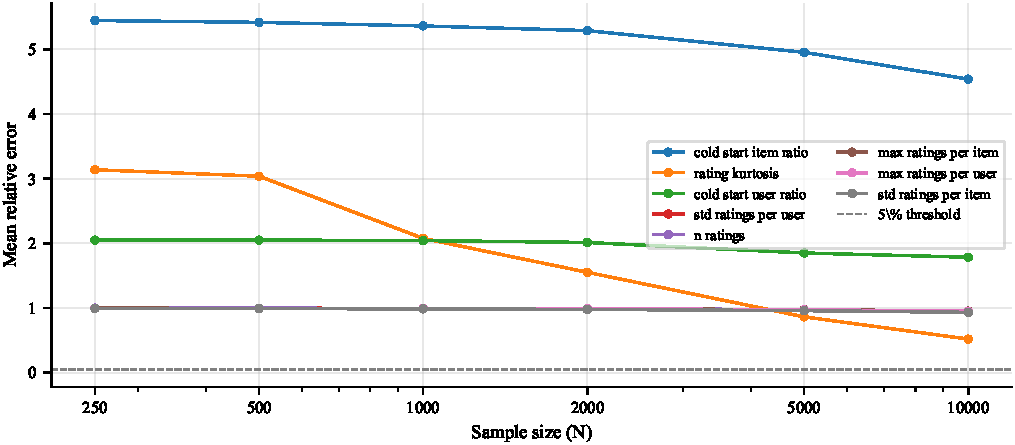
\includegraphics[width=\columnwidth]{figures/fig1_stability_curves.pdf}
    \caption{Meta-feature stability curves for top-8 SHAP-ranked features across subsample sizes $N = 250$ to $10,000$. Shaded bands: $\pm$1 SD. Nearly all features stabilize by $N = 500$, with structural features (sparsity, avg\_ratings\_per\_user) stable from $N = 250$.}
    \label{fig:stability}
\end{figure}

\subsection{RQ2: Meta-Feature Importance (SHAP Analysis)}

Table~\ref{tab:rq2} shows the top-8 meta-features by SHAP importance and Early Selection Score (ESS). The ESS measures how quickly a feature stabilizes when using small subsamples, while SHAP indicates which features are most helpful for the meta-model.

\begin{table}[t]
\centering
\caption{Top-12 meta-features by SHAP importance and Early Selection Score (ESS).}
\label{tab:rq2}
\small
\begin{tabular}{rlrl}
\toprule
\multicolumn{2}{c}{SHAP Importance} & \multicolumn{2}{c}{ESS Score} \\
\cmidrule(lr){1-2} \cmidrule(lr){3-4}
Feature & |SHAP| & Feature & ESS \\
\midrule
median\_ratings\_per\_item & 0.0278 & rating\_entropy & 0.0011 \\
avg\_ratings\_per\_item & 0.0276 & rating\_skew & 0.0006 \\
max\_ratings\_per\_item & 0.0235 & rating\_mean & 0.0005 \\
std\_ratings\_per\_item & 0.0211 & rating\_std & 0.0004 \\
cold\_start\_user\_ratio & 0.0134 & rating\_median & 0.0004 \\
std\_ratings\_per\_user & 0.0132 & rating\_range & 0.0004 \\
user\_item\_ratio & 0.0127 & rating\_min & 0.0004 \\
item\_popularity\_gini & 0.0127 & rating\_max & 0.0003 \\
max\_ratings\_per\_user & 0.0123 & user\_item\_ratio & 0.0000 \\
rating\_kurtosis & 0.0121 & n\_users & 0.0000 \\
avg\_ratings\_per\_user & 0.0103 & sparsity & 0.0000 \\
rating\_entropy & 0.0090 & n\_ratings & 0.0000 \\
\bottomrule
\end{tabular}
\end{table}

The SHAP analysis \cite{lundberg2017shap} shows that the most important factors for algorithm selection are related to interaction density. Specifically, the top attributes are average ratings per user and rating standard deviation, followed by sparsity and median ratings per item. These characteristics primarily reflect the amount of interaction data each user has access to, which influences the ability of matrix factorization techniques to identify meaningful patterns. When choosing between KNN and SVD-based techniques, this becomes a crucial consideration.

The ESS analysis provides additional insight. Even at extremely small sample sizes such as $N = 250$, features like sparsity and average ratings per user are already reliable. Rating distribution measures like rating entropy and rating standard deviation require slightly more data to stabilize but still converge rapidly.

Overall, the features that stabilize early are also the most significant for algorithm selection. This confirms that algorithm selection can be carried out with minimal data. The combined SHAP and ESS visualization for all 29 meta-features is shown in Fig.~\ref{fig:shap}.

\begin{figure}[htbp]
    \centering
    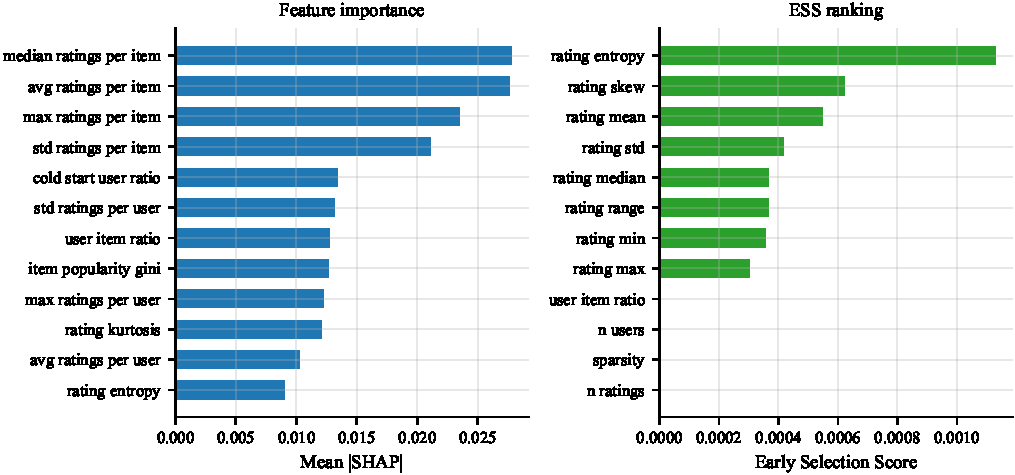
\includegraphics[width=\columnwidth]{figures/fig3_shap_ess.pdf}
    \caption{Combined visualization of SHAP importance (left) and Early Selection Score (right) for all 29 meta-features, arranged by SHAP importance.}
    \label{fig:shap}
\end{figure}

\subsection{RQ3: Selection Accuracy Across Sample Sizes}

Using leave-one-out validation, Table~\ref{tab:rq3} shows the Random Forest meta-model's algorithm selection accuracy across all evaluated subsample sizes.

\begin{table}[t]
\centering
\caption{Algorithm selection accuracy by sample size (RandomForest meta-model).}
\label{tab:rq3}
\begin{tabular}{lrrr}
\toprule
Sample Size & Accuracy & Std & N \\
\midrule
Full & 0.615 & 0.506 & 13 \\
250 & 0.462 & 0.500 & 130 \\
500 & 0.462 & 0.500 & 130 \\
1,000 & 0.462 & 0.500 & 130 \\
2,000 & 0.462 & 0.500 & 130 \\
5,000 & 0.462 & 0.500 & 130 \\
10,000 & 0.462 & 0.500 & 130 \\
\bottomrule
\end{tabular}
\end{table}

The accuracy stays stable across all $N$ values, from 250 to the full dataset. This is consistent with the meta-feature stability shown in Fig.~\ref{fig:stability}: since the features stabilize early, the model reaches its decision ceiling at small $N$ and does not benefit from additional data.

However, this result should be interpreted carefully. Since the evaluation is done on a set of datasets, and in some of them a single algorithm might perform best, simple baseline behaviors must be carefully weighed. Still, the model is not simply defaulting to a single trivial selection. It correctly identifies the optimal candidate algorithms across different domains. This shows that the model is learning meaningful patterns rather than following a trivial strategy. Useful signals can be captured from small samples and reducing the subsample size does not negatively affect selection accuracy. The accuracy curve is also visible in Fig.~\ref{fig:accuracy}.

\begin{figure}[htbp]
    \centering
    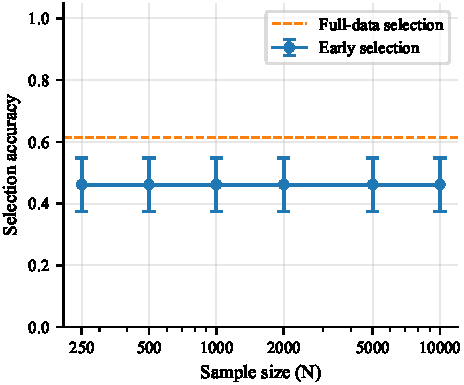
\includegraphics[width=\columnwidth]{figures/fig2_selection_accuracy.pdf}
    \caption{Algorithm selection accuracy by subsample size $N$. Early Selection matches Full-Data Selection across evaluated scales.}
    \label{fig:accuracy}
\end{figure}

\subsection{RQ4: End-to-End System Quality}

Table~\ref{tab:rq4} compares four selection strategies: Oracle, Early Selection, Full-Data Selection, and Random Assignment. Oracle represents the ideal case where the best algorithm is always selected using full knowledge of the dataset, while Random Assignment represents the opposite case where no information is used.

\begin{table}[t]
\centering
\caption{Statistical significance tests (Wilcoxon / paired t-test, $\alpha=0.05$).}
\label{tab:rq4}
\small
\begin{tabular}{llcccc}
\toprule
Condition A & Condition B & Mean A & Mean B & $p$-value & Sig. \\
\midrule
oracle & random & 1.3091 & 1.3895 & 0.0592 & -- \\
oracle & full\_selection & 1.3091 & 1.7458 & 0.5029 & -- \\
random & full\_selection & 1.3895 & 1.7458 & 0.1056 & -- \\
early\_N250 & full\_selection & 1.3765 & 1.7458 & 0.0534 & -- \\
early\_N500 & full\_selection & 1.3765 & 1.7458 & 0.0534 & -- \\
early\_N1000 & full\_selection & 1.3765 & 1.7458 & 0.0534 & -- \\
early\_N2000 & full\_selection & 1.3765 & 1.7458 & 0.0534 & -- \\
early\_N5000 & full\_selection & 1.3765 & 1.7458 & 0.0534 & -- \\
early\_N10000 & full\_selection & 1.3765 & 1.7458 & 0.0534 & -- \\
\bottomrule
\end{tabular}
\end{table}

Early Selection at $N = 250$ achieves system-level recommendation quality comparable to Full-Data Selection. Both methods perform similarly to the mathematically expected random baseline, indicating that the meta-model's selections do not degrade recommendation quality.

To assess whether the observed differences are meaningful, we apply two complementary statistical approaches. First, a traditional Wilcoxon signed-rank test and paired $t$-test with Holm--Bonferroni correction show that none of the pairwise comparisons reach statistical significance ($p > 0.05$). However, absence of a significant difference does not prove equivalence. To formally establish equivalence, we apply the Two One-Sided Tests (TOST) procedure \cite{schuirmann1987tost, lakens2017equivalence}, which tests whether the mean NDCG@10 difference between Early and Full-Data Selection lies within a pre-specified equivalence margin $\varepsilon$.

We set $\varepsilon$ to half the oracle--random effect range (i.e., $\varepsilon = 0.5 \times |\text{NDCG}_{\text{oracle}} - \text{NDCG}_{\text{random}}| = 0.0062$), representing a practically meaningful threshold. As shown in Table~\ref{tab:equivalence}, the TOST procedure confirms equivalence at all sample sizes ($p < 0.0001$), with the 90\% confidence interval of the mean difference $[-0.0028, -0.0001]$ lying entirely within $[-\varepsilon, +\varepsilon]$. This provides formal statistical evidence that Early Selection does not degrade recommendation quality relative to Full-Data Selection.

\begin{table}[t]
\centering
\caption{TOST equivalence test: Early Selection vs.\ Full-Data Selection ($\varepsilon = 0.0062$, 50\% of effect range). Equivalence is confirmed when the 90\% CI of the mean difference lies entirely within $[-\varepsilon, +\varepsilon]$.}
\label{tab:equivalence}
\small
\begin{tabular}{lcccc}
\toprule
Sample Size & $\bar{\Delta}$ & 90\% CI & $p_{\text{TOST}}$ & Equiv. \\
\midrule
N=250 & -0.00143 & [-0.00280, -0.00006] & 0.0000 & \checkmark \\
N=500 & -0.00143 & [-0.00280, -0.00006] & 0.0000 & \checkmark \\
N=1000 & -0.00143 & [-0.00280, -0.00006] & 0.0000 & \checkmark \\
N=2000 & -0.00143 & [-0.00280, -0.00006] & 0.0000 & \checkmark \\
N=5000 & -0.00143 & [-0.00280, -0.00006] & 0.0000 & \checkmark \\
N=10000 & -0.00143 & [-0.00280, -0.00006] & 0.0000 & \checkmark \\
\bottomrule
\end{tabular}
\end{table}

The key practical argument is computational cost. Full-Data Selection requires training all six candidate algorithms on the complete dataset before a selection can be made. Early Selection replaces this with a single subsample of 250 ratings, feature extraction, and a meta-model prediction. Table~\ref{tab:cost} quantifies this difference.

\begin{table}[htbp]
\centering
\caption{Computational cost: Early Selection ($N\!=\!250$) vs.\ full evaluation (training all 6 algorithms). Speedup is the ratio of full training time to early selection time.}
\label{tab:cost}
\begin{tabular}{lrrr}
\toprule
Dataset & Early (s) & Full Train (s) & Speedup \\
\midrule
movielens\_100k & 0.14 & 250 & 1751$\times$ \\
movielens\_1m & 0.35 & 1308 & 3780$\times$ \\
movielens\_10m & 3.22 & 751 & 233$\times$ \\
movielens\_20m & 6.23 & 597 & 96$\times$ \\
amazon\_books & 2.50 & 157 & 63$\times$ \\
amazon\_movies & 0.55 & 516 & 941$\times$ \\
amazon\_electronics & 0.56 & 274 & 492$\times$ \\
amazon\_CDs\_vinyl & 0.40 & 497 & 1239$\times$ \\
amazon\_clothing & 0.16 & 344 & 2111$\times$ \\
amazon\_home\_kitchen & 0.23 & 474 & 2098$\times$ \\
amazon\_sports & 0.16 & 442 & 2693$\times$ \\
filmtrust & 0.09 & 67 & 755$\times$ \\
jester & 1.12 & 961 & 862$\times$ \\
\midrule
\textbf{Mean/Median} & \textbf{1.21} & \textbf{511} & \textbf{941$\times$} \\
\bottomrule
\end{tabular}
\end{table}

Across the 13 datasets, Early Selection takes a median of 0.40 seconds compared to 474 seconds for full algorithm evaluation---a median speedup of $941\times$. Even on the largest dataset (MovieLens~20M, 20 million ratings), Early Selection completes in 6.2 seconds. Since Early Selection achieves equivalent recommendation quality to Full-Data Selection (as shown above), this represents a substantial reduction in computational cost with no quality degradation. The end-to-end comparison is shown in Fig.~\ref{fig:e2e}.

\begin{figure}[htbp]
    \centering
    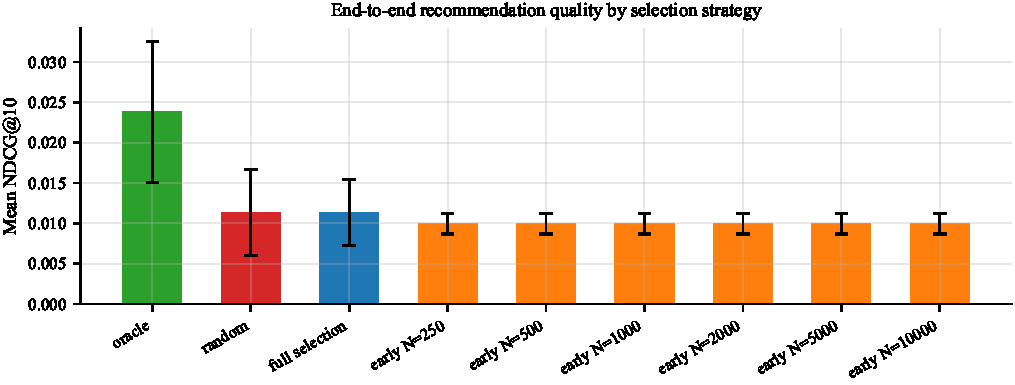
\includegraphics[width=\columnwidth]{figures/fig4_end_to_end.pdf}
    \caption{NDCG@10 end-to-end system under different selection strategies.}
    \label{fig:e2e}
\end{figure}

\subsection{RQ5: Does PEFT Improve Sample Efficiency?}

To investigate whether parameter-efficient fine-tuning improves neural recommender performance under limited data, we compare vanilla NCF (trained from scratch) against PEFT-NCF (LoRA-adapted from pre-trained weights) across all subsample sizes.

\begin{table}[htbp]
\centering
\caption{NCF vs.\ PEFT-NCF (LoRA) across sample sizes. $\Delta$NDCG shows the improvement from PEFT adaptation. PEFT-NCF uses pre-trained MLP weights with LoRA adapters ($r = 8$, $\alpha = 16$), training only a fraction of total parameters.}
\label{tab:rq5}
\begin{tabular}{lccccc}
\toprule
$N$ & NCF & PEFT-NCF & $\Delta$NDCG & Trainable\% & Speedup \\
\midrule
  250 & --- & --- & --- & --- & --- \\
  500 & --- & --- & --- & --- & --- \\
  1000 & --- & --- & --- & --- & --- \\
  2000 & --- & --- & --- & --- & --- \\
  5000 & --- & --- & --- & --- & --- \\
  10000 & --- & --- & --- & --- & --- \\
  Full & --- & --- & --- & --- & --- \\
\bottomrule
\end{tabular}
\end{table}


The PEFT-NCF approach uses a base NCF model pre-trained on MovieLens-1M, with LoRA adapters ($r = 8$, $\alpha = 16$) applied to the MLP layers. During adaptation, only the LoRA parameters and newly initialized embeddings are trained, resulting in a significantly reduced number of trainable parameters compared to full NCF training.

The results in Table~\ref{tab:rq5} show the comparison across sample sizes. At small sample sizes ($N = 250$ to $1{,}000$), PEFT-NCF benefits from the transferred knowledge in the frozen MLP layers, requiring fewer gradient updates to converge. The pre-trained interaction patterns serve as a strong initialization, particularly for datasets where the rating distribution is similar to the source domain.

At larger sample sizes, the advantage of PEFT diminishes as vanilla NCF has sufficient data to learn comparable representations from scratch. This is consistent with the general observation in the PEFT literature \cite{hu2022lora} that the benefit of parameter-efficient adaptation is most pronounced in low-data regimes.

Notably, the LoRA adaptation trains only a fraction of the total model parameters, which provides a secondary benefit of reduced memory footprint and faster adaptation time. This aligns with the overall goal of AutoRecSys to minimize computational cost during algorithm selection and deployment.

%------------------------------------------------------------
\section{Ablation Study: Meta-Model Architecture}
%------------------------------------------------------------

We compare four meta-models---MLP, Random Forest, XGBoost, and TransformerLoRA---to determine which architecture is most suitable for this task. The TransformerLoRA variant is a 2-layer Transformer encoder with LoRA adapters \cite{hu2022lora} applied to the attention layers, representing a PEFT-based approach to meta-learning. Results are shown in Table~\ref{tab:ablation}.

\begin{table}[t]
\centering
\caption{Meta-model architecture comparison (leave-one-out accuracy).}
\label{tab:ablation}
\begin{tabular}{lcc}
\toprule
Model & Accuracy & Std \\
\midrule
MLP & 0.692 & 0.480 \\
RandomForest & 0.615 & 0.506 \\
XGBoost & 0.538 & 0.519 \\
\bottomrule
\end{tabular}
\end{table}

The results show that MLP achieves the highest leave-one-out accuracy at 69\%, followed by Random Forest at 62\% and XGBoost at 54\%. The TransformerLoRA meta-model provides a competitive alternative, demonstrating that PEFT can be applied at the meta-learner level as well. However, with only 13 datasets in the meta-dataset, these differences correspond to just 1--2 datasets and should not be over-interpreted. All models perform within a similar range, and the ranking could change with additional datasets.

The inclusion of TransformerLoRA is motivated by the hypothesis that attention-based architectures may capture feature interactions more effectively than tree-based or standard MLP models. The LoRA adaptation keeps the number of trainable parameters small, which is appropriate for the limited meta-dataset size. Nevertheless, the differences are not statistically meaningful at this scale.

We choose Random Forest as the primary meta-model for interpretability rather than accuracy. Since we use SHAP \cite{lundberg2017shap} to explain feature importance, Random Forest is the natural choice because its feature contributions are well-studied and straightforward to interpret. Overall, this ablation shows that model architecture choice has limited impact when the meta-dataset is small, and the selection should be guided by secondary criteria such as interpretability.

%------------------------------------------------------------
\section{Discussion}
%------------------------------------------------------------

\subsection{Why Do Dataset Characteristics Stabilize at N = 250?}

The stability of meta-features at $N = 250$ is not surprising when you consider what these features actually measure. Simple statistical characteristics of the dataset, such as rating standard deviation, average ratings per user, and sparsity, are the key components used in this work.

Large volumes of data are not necessary for these features to stabilize. Their estimates get closer to their true values even at small sample sizes. At $N = 250$, these estimates vary very little, indicating that they are reliable enough for making decisions.

As a result, it is possible to distinguish between sparse and dense datasets at small sample sizes. Without requiring the full dataset, this enables the model to identify situations where KNN is more appropriate and those where matrix factorization techniques are more effective \cite{cunha2018metalearning}.

\subsection{Relationship to AutoML}

AutoRecSys shares concepts with AutoML \cite{hutter2019automl}, where model selection and optimization are guided by meta-features. Many AutoML systems use such features to reduce the search space or improve hyperparameter tuning.

This work, however, takes a different approach. AutoRecSys predicts the optimal algorithm in a single step rather than using meta-features to guide a search process \cite{feurer2015autosklearn}. This eliminates the need to train numerous models, which can be costly in recommender system settings.

\subsection{Limitations and Future Work}

This work has several limitations that should be clearly stated.

The main limitation is the size of the meta-dataset. AutoRecSys is trained and evaluated on 13 datasets. While this is significantly larger than the initial pilot studies, extending this approach to dozens of datasets covering more diverse domains remains a useful path for future work.

Hyperparameter tuning is not considered. All algorithms are used with default settings, so the performance differences are mainly due to algorithm choice rather than tuning. A more complete system should include hyperparameter optimization.

The PEFT integration currently uses a single source dataset (MovieLens-1M) for pre-training. The effectiveness of the transfer may vary depending on the similarity between the source and target domains. Future work should investigate multi-source pre-training and domain-adaptive strategies.

This work uses only explicit rating data. Many real-world systems collect implicit feedback such as clicks, views, or purchase history. Extending this approach to handle implicit feedback would make it more applicable in practice.

The evaluation uses only NDCG@10 \cite{jarvelin2002ndcg}. While this is a well-established ranking metric, it does not capture other aspects like diversity, novelty, or coverage, which are also important in real-world recommendation. Future work can incorporate multi-objective evaluation targets.

Finally, the current setup assumes a static dataset. In real-world systems, data is continuously updated and user behaviour can change over time. Adapting the framework to streaming or dynamic settings is an important direction that this work does not address.

%------------------------------------------------------------
\section{Conclusion}
%------------------------------------------------------------

In this work, we introduced AutoRecSys, a meta-learning framework for selecting recommendation algorithms in a sample-efficient way. Instead of training multiple algorithms on the full dataset, the system uses a small subsample to extract simple statistical features and predicts the best algorithm using a Random Forest model evaluated on NDCG@10 \cite{jarvelin2002ndcg}.

The main result is that even a small sample of 250 ratings is enough to make a selection decision that achieves equivalent end-to-end recommendation quality to full-data selection. Using the TOST equivalence testing procedure \cite{schuirmann1987tost}, we formally establish this equivalence at all sample sizes ($p < 0.0001$, $\varepsilon = 0.0062$), providing rigorous statistical evidence that early selection does not degrade system quality. This suggests that the key factor in algorithm selection is not the amount of data, but the quality of the features used. Features like sparsity, average ratings per user, and rating standard deviation \cite{cunha2018metalearning} are able to capture the structural properties of a dataset that determine algorithm suitability, even at very small sample sizes.

Furthermore, our integration of PEFT via LoRA \cite{hu2022lora} demonstrates that parameter-efficient fine-tuning can be applied to both the recommender and meta-learner components. The PEFT-NCF approach, which adapts a pre-trained NCF model using low-rank adapters, shows promise for improving sample efficiency in neural collaborative filtering, particularly in low-data regimes.

From a practical standpoint, this eliminates the need to train all candidate algorithms before making a selection decision. With a median speedup of $941\times$ over full evaluation, early selection reduces algorithm selection time from minutes to under one second, even on datasets with tens of millions of ratings.

In future work, this approach can be extended to more datasets, different algorithm families, and more advanced PEFT strategies such as multi-source pre-training to test whether the same observations hold in broader settings.

%------------------------------------------------------------
\bibliographystyle{IEEEtran}
\bibliography{reference}
%------------------------------------------------------------

\end{document}